%------------------------------------------------------------------------------------
%	PACKAGES AND OTHER DOCUMENT CONFIGURATIONS
%------------------------------------------------------------------------------------

\documentclass{article}

\usepackage{fancyhdr} % Required for custom headers
\usepackage{lastpage} % Required to determine the last page for the footer
\usepackage{extramarks} % Required for headers and footers
\usepackage[usenames,dvipsnames]{color} % Required for custom colors
\usepackage{graphicx} % Required to insert images
\usepackage{subcaption}
\usepackage{listings} % Required for insertion of code
\usepackage{courier} % Required for the courier font
% Optional Packages
\usepackage{amsmath}
\usepackage{amssymb}
\usepackage{float}
\usepackage{algorithm}
\usepackage[noend]{algpseudocode}


% Margins
\topmargin=-0.45in
\evensidemargin=0in
\oddsidemargin=0in
\textwidth=6.5in
\textheight=9.0in
\headsep=0.25in

\linespread{1.1} % Line spacing

% Set up the header and footer
\pagestyle{fancy}
\lhead{\hmwkAuthorName} % Top left header
\chead{\hmwkClass\ : \hmwkTitle} % Top center head
%\rhead{\firstxmark} % Top right header
\lfoot{\lastxmark} % Bottom left footer
\cfoot{} % Bottom center footer
\rfoot{Page\ \thepage\ of\ \protect\pageref{LastPage}} % Bottom right footer
\renewcommand\headrulewidth{0.4pt} % Size of the header rule
\renewcommand\footrulewidth{0.4pt} % Size of the footer rule

\setlength\parindent{0pt} % Removes all indentation from paragraphs


%------------------------------------------------------------------------------------
%	DOCUMENT STRUCTURE COMMANDS
%	Skip this unless you know what you're doing
%------------------------------------------------------------------------------------

% Header and footer for when a page split occurs within a problem environment
\newcommand{\enterProblemHeader}[1]{
	%\nobreak\extramarks{#1}{#1 continued on next page\ldots}\nobreak
	%\nobreak\extramarks{#1 (continued)}{#1 continued on next page\ldots}\nobreak
}

% Header and footer for when a page split occurs between problem environments
\newcommand{\exitProblemHeader}[1]{
	%\nobreak\extramarks{#1 (continued)}{#1 continued on next page\ldots}\nobreak
	%\nobreak\extramarks{#1}{}\nobreak
}

\setcounter{secnumdepth}{0} % Removes default section numbers
\newcounter{homeworkProblemCounter} % Creates a counter to keep track of the number of problems
\setcounter{homeworkProblemCounter}{0}

\newcommand{\homeworkProblemName}{}
\newenvironment{homeworkProblem}[1][Problem \arabic{homeworkProblemCounter}]{ % Makes a new environment called homeworkProblem which takes 1 argument (custom name) but the default is "Problem #"
	\stepcounter{homeworkProblemCounter} % Increase counter for number of problems
	\renewcommand{\homeworkProblemName}{#1} % Assign \homeworkProblemName the name of the problem
	\section{\homeworkProblemName} % Make a section in the document with the custom problem count
	\enterProblemHeader{\homeworkProblemName} % Header and footer within the environment
}{
	\exitProblemHeader{\homeworkProblemName} % Header and footer after the environment
}

\newcommand{\problemAnswer}[1]{ % Defines the problem answer command with the content as the only argument
	\noindent\framebox[\columnwidth][c]{\begin{minipage}{0.98\columnwidth}#1\end{minipage}} % Makes the box around the problem answer and puts the content inside
}

\newcommand{\homeworkSectionName}{}
\newenvironment{homeworkSection}[1]{ % New environment for sections within homework problems, takes 1 argument - the name of the section
	\renewcommand{\homeworkSectionName}{#1} % Assign \homeworkSectionName to the name of the section from the environment argument
	\subsection{\homeworkSectionName} % Make a subsection with the custom name of the subsection
	\enterProblemHeader{\homeworkProblemName\ [\homeworkSectionName]} % Header and footer within the environment
}{
	\enterProblemHeader{\homeworkProblemName} % Header and footer after the environment
}


%=================================================================

%------------------------------------------------------------------------------------
%	NAME AND CLASS SECTION
%------------------------------------------------------------------------------------

\newcommand{\hmwkTitle}{Assignment\ \#3} % Assignment title
\newcommand{\hmwkClass}{CSC 411} % Course/class
\newcommand{\hmwkAuthorName}{Xiangyu Kong \hspace{3em} Yun Lu} % Your name
\newcommand{\hmwkUTorId}{kongxi16 \hspace{5em} luyun5} % UTorID

%------------------------------------------------------------------------------------
%	TITLE PAGE
%------------------------------------------------------------------------------------

\title{
	\vspace{2in}
	\textmd{\textbf{\hmwkClass:\ \hmwkTitle}}\\
	%	\normalsize\vspace{0.1in}\small{Due\ on\ \hmwkDueDate}\\
	\vspace{0.1in}
	\vspace{3in}
}

\author{\textbf{\hmwkAuthorName} \\ \textbf{\hmwkUTorId}}

% Insert date here if you want it to appear below your name
\date{\today}

%------------------------------------------------------------------------------------

\begin{document}
	
	\maketitle
	\clearpage
	
	%---------------------------------------------------------------------------------
	%	PROBLEM 1
	%---------------------------------------------------------------------------------
	\begin{homeworkProblem}
		%		\noindent \textit{Question}
		The dataset contains headlines including the word ``Trump". The quality of the dataset is generally good since there is a large variety of vocabularies included. \\
		
		By observing, we can see that the fake news' headlines are generally longer than the real news' headlines. \\
		
		Except for ``Donald" and ``Trump", the most frequent words are ``to", ``for", etc, but they do not mean a lot. The top meaningful words in total are ``Clinton", ``election" and ``president".  This infers that most news are regarding the 2017 presidential election and especially between Donald Trump and Hilary Clinton.\\
		
		The statistics for the three words are generated through part1 in fake.py and the results are given below in Listing 1. We can see that although ``Clinton" has the largest word count, most of them appear in the fake news. Reports that include ``election" are more likely to be real news. \\
		
		\begin{lstlisting}[caption=statistic results]
		[clinton]:
			real: 83
			fake: 132
			total: 215
		[election]:
			real: 87
			fake: 74
			total: 161
		[president]:
			real: 66
			fake: 64
			total: 130
		\end{lstlisting}
		
	\end{homeworkProblem}
	\clearpage
	
	%---------------------------------------------------------------------------------
	
	%---------------------------------------------------------------------------------
	%	PROBLEM 2
	%---------------------------------------------------------------------------------
	\begin{homeworkProblem}
		%		\noindent \textit{Question}
		The Naive Bayes algorithm is implemented in naive\_bayes in util.py. To tune the parameters $m$ and $\hat{p}$, we try using naive bayes on different value of $m$ and $\hat{p}$ and pick one that has the best performance on the validation set. The range of test values for $m$ was from 1 to 10, and for $\hat{p}$ was from 0.05 to 0.95. The returned optimum values were $m = 1$ and $\hat{p} = 0.25$.\\
		
		To deal with small multiplication, a small\_product function was implemented in util.py. It takes in a list of small values and uses the fact that $\prod \limits_{i = 1}^{N} a_i = \exp (\sum \limits_{i = 1}^{N} \log(a_i))$ to compute the value of $p(a_1, a_2, \dots, a_n) = p(a_1) p(a_2) \dots p(a_1)$\\
		
		The performance on training set, validation set and test set is given below:
		
		\begin{lstlisting}[caption = Performance]
	train performance = 0.964597902098
	validation performance = 0.842535787321
	test performance = 0.881390593047
		\end{lstlisting}
		
	\end{homeworkProblem}
	\clearpage
	
	%---------------------------------------------------------------------------------
		
	%---------------------------------------------------------------------------------
	%	PROBLEM 3
	%---------------------------------------------------------------------------------
	\begin{homeworkProblem}
		%		\noindent \textit{Question}
		\begin{enumerate}
			\item 
			The results are produced by part3 in fake.py and are listed below. \\
			
			$P(c | word) = \dfrac{P(word | c) \times P(c)}{P(words)}$ where \\$P(c) = \dfrac{count(c)}{count(total)}$, $P(word | c) = \dfrac{count(word\ in\ c)}{count(c)}$ and $P(word) = \dfrac{count(word\ in\ c)}{count(total)}$\\
			
			$P(c | not\ word)$ follows with similar calculations.\\
			
			The most important presence for predicting a class means $P(c | word)$ must be high and the most important absence for predicting a class means $P(c | not\ word)$ must be high.\\
			
			\item 
			After removing the stop words like ``to", ``us", ``in", and etc,  we get the results in b.
			
			\item 
			The stop words are very likely to appear no matter what class the headline is, so including them will not mean a lot.
		\end{enumerate}
	
		\begin{lstlisting}[caption = top results]
	a:
	Real: 
	top 10 important presence: 
		['trump', 'donald', 'to', 'us', 'trumps', 'in', 'on', 
		'of', 'says', 'for']
	top 10 important absence: 
		['kommonsentsjane', 'lord', 'tired', 'miller', '270',
		 'elegant', 'battleground', 'fingers', 'salbuch', 'cult']
	Fake:
	top 10 important presence: 
		['trump', 'to', 'the', 'donald', 'in', 'of', 'for', 'a', 'and', 'on']
	top 10 important absence: 
		['hanging', 'marching', 'regional', 'hearin', 'piling', 
		'jennett', 'loathing', 'deferred', 'decry', 'lgbt']
	
	b:
	Real: 
	top 10 important presence: 
		['trump', 'donald', 'trumps', 'says', 'election', 
		'clinton', 'north', 'korea', 'ban', 'president']
	Fake:
	top 10 important presence: 
		['trump', 'donald', 'hillary', 'clinton', 'election', 
		'just', 'new', 'president', 'obama', 'america']
		
		\end{lstlisting}
		
	\end{homeworkProblem}
	\clearpage
	
	%---------------------------------------------------------------------------------
		
	%---------------------------------------------------------------------------------
	%	PROBLEM 4
	%---------------------------------------------------------------------------------
	\begin{homeworkProblem}
		%		\noindent \textit{Question}
		The logistic regression is implemented in logistic\_regression.py. The parameters $\alpha$ and $\lambda$ are selected using the similar method as in Problem 2. The two parameters were assigned to various values and the optimum value is the pair where the validation set performs the best. The final $\alpha = 0.0001$ and $\lambda = 0.001$.
		
		Using this pair of parameters, the final logistic regression model gives the learning curve as in Fig.\ref{fig:4.1}. 
		
		\begin{figure}[!ht]
			\centering
			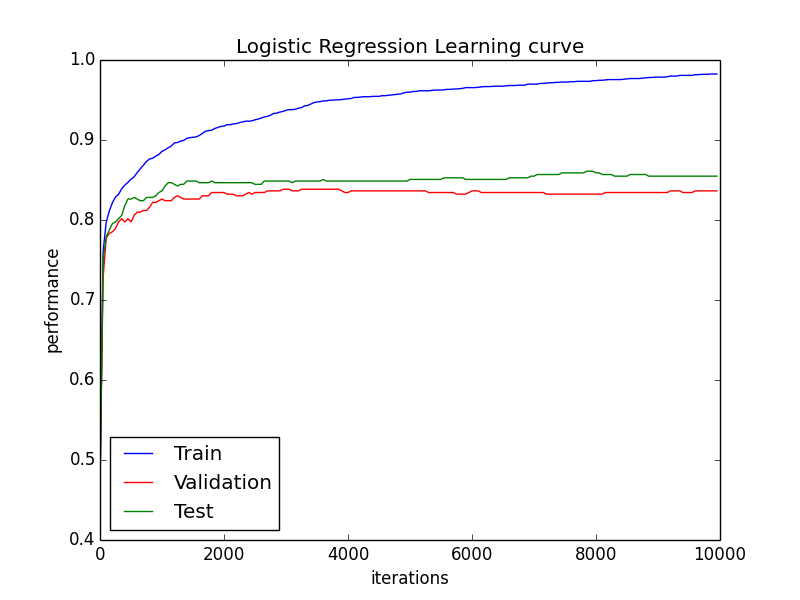
\includegraphics[width=.75\linewidth]{images/4/learning_curve.png}
			\caption{caption}
			\label{fig:4.1}
		\end{figure}
		
	\end{homeworkProblem}
	\clearpage
	
	%---------------------------------------------------------------------------------
		
	%---------------------------------------------------------------------------------
	%	PROBLEM 5
	%---------------------------------------------------------------------------------
	\begin{homeworkProblem}
		
		For Naive Bayes, $\theta_0 = P(c)$, and $\theta_i = P(w_i , c)$ and $I_i(x) = \dfrac{1}{P(w_i)}$. The calculated result is $\dfrac{P(c | w_i)}{P(w_i)} $ but $w_i$ does not matter here so when the calculated value is greater than a threshold, we can say that the word combination is likely to produce a real or fake headline.\\
		
		For Logistic Regression, $\theta_i$s are the weights in the network. $I_i$s are the identity function that indicates whether the word $w_i$ is present. If the calculated output is greater than a specific threshold, then the output will be real.
		
	\end{homeworkProblem}
	\clearpage
	
	%---------------------------------------------------------------------------------
		
	%---------------------------------------------------------------------------------
	%	PROBLEM 6
	%---------------------------------------------------------------------------------
	\begin{homeworkProblem}
		%		\noindent \textit{Question}
		\begin{enumerate}
			\item 
			The results for the top positive and negative weight words are given in the list below (a). Comparing to the top important presence and absence word list in Problem 3a, the two lists have a few common words, but Problem 3a's list contains more stop words while the list given below has less stop words.
			
			\item 
			The list of words that do not include stop words are given in b.  Comparing to the top important presence and absence word list in Problem 3b, the two lists have a few common words, but they appear to be in different order. This shows that the two methods weigh the same word differently. 
			
			\item 
			When using logistic regression, if the features are not normalized, some features may have way more weight than other features. If the feature is very important, the magnitude of the feature will be very large thus affect the overall performance and cost.
			
			For this question, using the magnitude of the logistic regression parameters to indicate importance of a feature makes sense since we are performing binary classification here. The magnitude of the feature only decides whether the news is real or not. If there are more than two classes, using the magnitude of the parameters to indicate importance would be a mistake.
			
		\end{enumerate}
		
		\begin{lstlisting}[caption = Top positive and negative words]
	a:
	Positive:
	['trumps', 'australia', 'us', 'turnbull', 'tax', 'korea', 'ban', 
	'donald', 'debate', 'administration']
	Negative:
	['hillary', 'victory', 'breaking', 'just', 'watch', 'information', 
	'u', 'are', 'd', 'soros']
	b:
	Positive:
	['trumps', 'australia', 'turnbull', 'tax', 'korea', 'ban', 'donald', 
	'debate', 'administration', 'says']
	Negative:
	['hillary', 'victory', 'breaking', 'just', 'watch', 'information', 'u', 
	'd', 'soros', 'won']
		\end{lstlisting}
		
	\end{homeworkProblem}
	\clearpage
	
	%---------------------------------------------------------------------------------
		
	%---------------------------------------------------------------------------------
	%	PROBLEM 7
	%---------------------------------------------------------------------------------
	\begin{homeworkProblem}
		%		\noindent \textit{Question}
		\begin{enumerate}
			\item 
			The relationship between the maximum depth of the decision tree and its performance is shown in Fig\ref{fig:7.1}. To generate the graph, the depth was chosen to be from range(1, 300, 30). As we can see, the graph looks similar to the learning rate graph in gradient descent. 
			
			The best performing depth was chosen to be {151} because it has the highest validation performance.
			
			Except for the max\_depth, the criterion parameter was chosen to be 'entropy' while constructing the tree. This is to relate to the following questions.
			
			\item 
			The visualization of the best decision tree above is given in Fig\ref{fig:7.2}.
			
			We can see that all the words in the first two layer of the decision tree are in the list of important words in part 3.
			
			\item 
			The performance of three methods are given in the table below. We can see that Naive Bayes has the highest validation and test result. Decision Tree has the best training result (100\%), but the lowest validation and test result. This is because it over-fits the data too much. 
			
			\begin{table}[h!]
				\centering
				\begin{tabular}{||c || c | c | c||} 
					\hline
					Method & Train & Validation & Test \\ [0.5ex] 
					\hline\hline
					Naive Bayes & 96.46 & 84.25 & 88.14 \\ 
					\hline
					Logistic Regression & 97.90 & 84.05 & 84.66 \\
					\hline
					Decision Tree & 100 & 76.07 & 78.32 \\
					\hline
				\end{tabular}
			\end{table}
			
		\end{enumerate}
		
		\begin{figure*}[!ht]
		
			\begin{subfigure}{.45\linewidth}
				\centering
				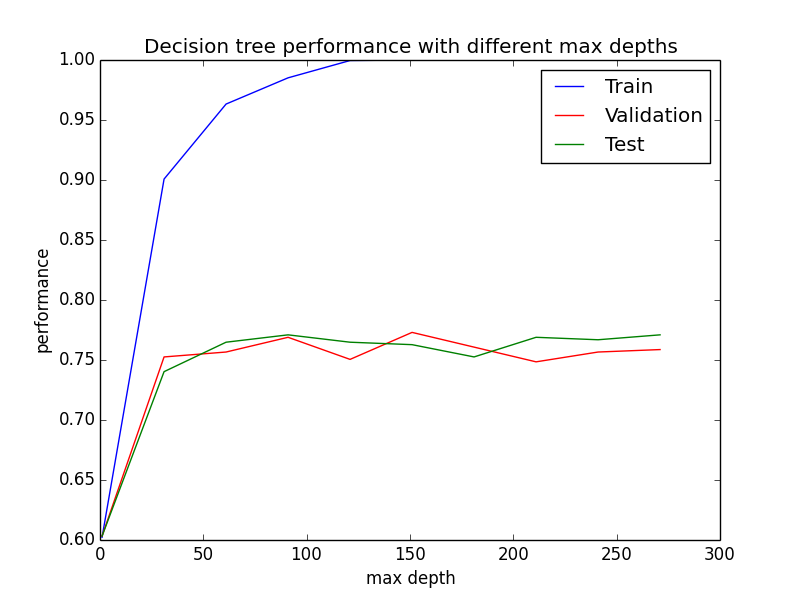
\includegraphics[width=\linewidth]{images/7/dt_performance.png}
				\caption{Learning Curve}
				\label{fig:7.1}
			\end{subfigure}
			\begin{subfigure}{.45\linewidth}
				\centering
				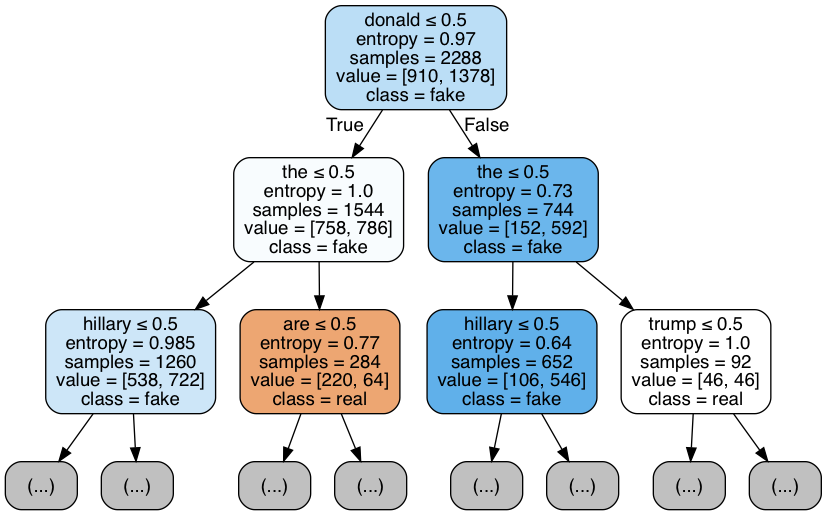
\includegraphics[width=\linewidth]{images/7/tree.png}
				\caption{Decision Tree}
				\label{fig:7.2}
			\end{subfigure}

		\end{figure*}
		
		
		
	\end{homeworkProblem}
	\clearpage
	
	%---------------------------------------------------------------------------------
		
	%---------------------------------------------------------------------------------
	%	PROBLEM 8
	%---------------------------------------------------------------------------------
	\begin{homeworkProblem}
	
		\begin{enumerate}
			\item 
			The first split of the tree is on the word $x_i$: ``donald". Through the following calculations, we get that:
			
			\begin{align*}
			H(Y) &= -P(Y = real) \log (P(Y = real)) + -P(Y = fake) \log (P(Y = fake)) = 0.967\\
				&= -\dfrac{910}{2288} \times \log(\dfrac{910}{2288}) - \dfrac{1378}{2288} \times \log( \dfrac{1378}{2288})\\
				&= 0.967\\
			H(Y | x_i) &= P(x_i = 0) H(Y | x_i = 0) + P(x_i = 1) H(Y | x_i = 1)\\
				&= \dfrac{1544}{2288} \times 1 + \dfrac{744}{2288} \times 0.73\\
				&= 0.911\\
			I(Y; x_i) &= H(Y) - H(Y | x_i) = 0.056\\
			\end{align*}
			
			\item 
			The second split word $x_j$ is chosen to ``the". Through the following calculations, we get that:
			\begin{align*}
			H(Y | x_j = 1) &= - (\dfrac{644}{1912} \times \log(\dfrac{644}{1912})) - (\dfrac{1268}{1912} \times \log(\dfrac{1268}{1912}))\\
				&= 0.921\\
			H(Y | x_j = 0) &= - (\dfrac{266}{376} \times \log(\dfrac{266}{376})) - (\dfrac{110}{376} \times \log(\dfrac{110}{376}))\\
				&= 0.871\\
			H(Y | x_j) &= \dfrac{1912}{2288} \times 0.921 + \dfrac{376}{2288} \times 0.871\\
				&= 0.913
			\end{align*}
			
			Then 
			\begin{align*}
				I(Y, x_j) = 0.967 - 0.913 = 0.054
			\end{align*}
			
			This value is very close to the value we computed in 8(a), but it is still smaller. This is because these two words are very close and if this word has a larger information gain than x\_i, this word should be the first word to split the tree.
		\end{enumerate}
	
	\end{homeworkProblem}
	\clearpage
	
	%---------------------------------------------------------------------------------
\end{document}